\documentclass[11pt, english, fleqn, DIV=15, headinclude, BCOR=2cm]{scrreprt}

\usepackage[
    color,
    bibatend,
]{../../header}

\graphicspath{{./}{../Figures/}}

\newcommand\MZ{M_{\mathrm Z^0}}
\newcommand\electron{\mathrm e^-}
\newcommand\positron{\mathrm e^+}

\usepackage{needspace}

\usepackage{mathtools}
\usepackage{listings}

\lstset{
    basicstyle=\small\ttfamily,
}

\hypersetup{
    pdftitle=
}

\usepackage{longtable}
\usepackage{subcaption}

\usepackage[all]{nowidow}

\subject{Lab report}
\title{Positron lifetime in metals and insulators}
\subtitle{Experiment K225 -- Universität Bonn}
\author{%
    Martin Ueding \\
    \small{\href{mailto:mu@martin-ueding.de}{mu@martin-ueding.de}}
    \and
    Lino Lemmer \\
    \small{\href{mailto:l2@uni-bonn.de}{l2@uni-bonn.de}}
}

\date{\daterange{2016-03-24}{2016-03-25}}

\publishers{Tutor: Martin Urban}

\begin{document}

\maketitle

\begin{abstract}
        In this experiment we use a fast-slow-coincidence circuit to measure
        the temperature dependence of the positron lifetime in metals. Due to
        different lifetimes of free and trapped positrons we can examine the
        formation of vacancies in the metal. 
        
        In an overnight measurement we determine the lifetimes of free and
        trapped positronium in an insulator. 
\end{abstract}

\tableofcontents

\chapter*{Permission to upload}

I, Martin Ueding, would like to scan and upload this lab report with your
corrections to my website \href{http://martin-ueding.de}{martin-ueding.de}.
There, the original lab report as well as the reviewed one will be licensed
under the “\href{http://creativecommons.org/licenses/by-sa/4.0/}{Creative
Commons Attribution-ShareAlike 4.0 International License}”. Is that okay with
you?

Yes $\Box$ \hspace{2cm} No $\Box$

\chapter{Theory}

\section{Positrons}

\subsection{Positron sources}

Our source of positrons will be $\mathrm{^{22}Na}$ throughout the experiment.
Figure~\ref{fig:na22} shows that the sodium decays via a $\betaup^+$-decay or
electron capture into an excited neon isotope. Both decay mechanism are related
via the crossing symmetry and have the same amplitude. Figure~\ref{fig:beta}
shows the first variant. The excited neon will quickly decay into the ground
state and emit a photon. Said photon will mark the creation of the positron.

\begin{figure}
    \centering
    \includegraphics{na22}
    \caption{%
        Decay of $\mathrm{^{22}Na}$.
    }
    \label{fig:na22}
\end{figure}

Due to the creation of the neutrino, the energy spectrum of the positron is
continuous.

\begin{figure}
    \centering
    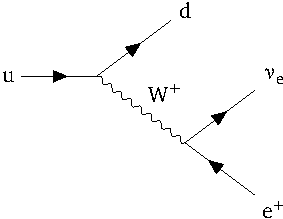
\includegraphics{beta}
    \caption{%
        Feynman diagram for the $\betaup^+$-decay.
    }
    \label{fig:beta}
\end{figure}

\subsection{Positron annihilation}
\label{ssec:pos_ann}

The tree-level annihilation diagrams are shown in
Figure~\ref{fig:annihilation}. Depending on the relative spin orientations of
the electron and positron, a decay into an even or odd number of photons is
possible. The decay into a single photon is not possible due to
energy-momentum-conservation. Also, the additional creation of two more photon
suppresses the cross section by $\alpha \approx 1/137$. Therefore we can assume
that only decays in two and three photons occur.

\begin{figure}
    \centering
    \begin{subfigure}[c]{0.48\linewidth}
        \centering
        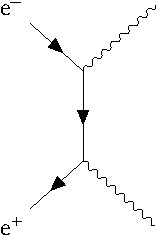
\includegraphics{two-photon}
        \caption{%
            Two photons
        }
        \label{fig:/1}
    \end{subfigure}
    \hfill
    \begin{subfigure}[c]{0.48\linewidth}
        \centering
        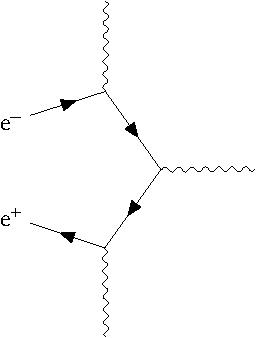
\includegraphics{three-photon}
        \caption{%
            Three photons
        }
        \label{fig:/2}
    \end{subfigure}
    \caption{%
        Decay of a positron into photons.
    }
    \label{fig:annihilation}
\end{figure}

\subsection{Positronium formation}

A positron can form a hydrogen-like metastable bound state with an electron.
Depending on the particle's spins this state is called para-positronium (spins
antiparallel) or ortho-positronium (spins parallel). The positronium atom will
decay eventually due to a finite possibility for the positron to be located at
the electron's position and vice versa. As written in
Section~\ref{ssec:pos_ann} the para-positronium only decays in two photons and
the ortho-positronium only in three photons. If the latter is located near
other atoms, the long lifetime leads to the so called pick-off process, where
the positron annihilates with one of the atom's electrons with antiparallel
spin. This again leads to a reduced lifetime, which still is remarkably longer
than the para-positronium's one.

\section{Metals}

A perfect metal consists of only atoms of one type. They are arranged in a
perfect periodic lattice, usually a Bravais lattice with a trivial unit cell.
Some electrons can move rather freely between the atoms as their wave functions
are mostly delocalized in the conducting band.

\subsection{Lattice defects}

In reality, the perfect periodic lattice is not realized. There are other atoms
in the lattice, taking a regular lattice site. Those foreign atoms might be
larger or smaller than the regular atoms. The number of electrons can be
different for such a foreign atom. In doped semiconductors, this is
deliberately done to obtain certain electronic properties.

There are also mesoscopic lattice defects like shifts, tears or similar
disruptions to the periodicity. At the surfaces where such a shift happen,
the distance between the atoms becomes very irregular.

\subsection{Vacancies}

The lattice might be disturbed in a way which leaves gaps in the lattice, sites
are not filled with an atom. Those spots are called vacancies. There, electrons
neighboring atoms aggregate as there is no repelling positive charge.

The density of vacancies depends on the temperature. The higher the
temperature, the more vacancies we expect. At temperature $T$, the density of
vacancies is given by \textcite[(3)]{Weiler/Vacancy_formation} as
\[
    C(T) = \exp\del{\frac{S}{k}} \exp\del{-\frac{H_\mathrm t}{kT}} \,.
\]
$H_\mathrm t$ is the energy needed for a vacancy to form, it is called
\enquote{vacancy formation enthalpy}.

\subsection{Trapping model}
\label{ssec:tra_mod}

In a metal, the amount of free electrons is very large. A positron cannot form
positronium as the amount of competing electrons is too high. The positron can
still come to rest in a vacancy as the net negative charge there will attract
and trap it.

Our trapping model is simple: Positrons can either be free and move through the
metal (Bloch wave) or be trapped in one of the vacancies. The lifetime for both
states is different, a free positron will have more opportunity to annihilate
than one in a vacancy with less electron density.

A trapped positron could become free again. In our experiment we will not see
this as the positron will annihilate before becoming free again. The model can
therefore be described by a free lifetime, a trapping rate and a trapped
lifetime.

As a free positron can either annihilate or become trapped, its total lifetime
is
\[
    \tau_0 = \del{\frac{1}{\tau_\mathrm f} + \sigma_\mathrm t C_\mathrm t}\inv
\]
as given by \textcite[(1a)]{Weiler/Vacancy_formation}.

The trapped lifetime simply is $\tau_\mathrm t$.

In an insulator, there is no conducting band of electrons. Positrons can
actually find an electron and form positronium with it. 

\section{Measurement technique}

\subsection{LYSO scintillator}

In order to detect the photons, we use a LYSO scintillator. This material is
radioactive itself and provides a built-in energy calibration. The decay scheme
of the radionuclide is shown in Figure~\ref{fig:scheme-176Lu}.

\begin{figure}
    \centering
    \includegraphics{scheme-176Lu}
    \caption{%
        Decay scheme of $^{176}\mathrm{Lu}$ into $^{176}\mathrm{Hf}$.
    }
    \label{fig:scheme-176Lu}
\end{figure}

Photons interact with matter through three main channels: photo effect, Compton
effect and pair production. In the case of the scintillation material, we are
not really interested in the details but use that usually the full energy of
the incident photon is deposited. The material will exhibit a light pulse which
is proportional to the incident energy.

\subsection{Photomultiplier}

The light pulse from the scintillator is too faint to measure directly. It is
therefore amplified with a photomultiplier. A schematic is shown in
Figure~\ref{fig:photomultiplier}. Incoming photons will free an electron via
the photo effect. The electron is then accelerated via several electric fields.
Once it hits the first dynode, the accelerated electron has enough energy to
create an avalanche of secondary electrons. This process repeats along the
dozen dynodes until a measurable current is created.

\begin{figure}
    \centering
    \includegraphics{photomultiplier}
    \caption{%
        %
    }
    \label{fig:photomultiplier}
\end{figure}

The signal at the very end of the multiplier might be saturated and have lost
its energy proportionality. This signal will rise very fast due to quick
saturation, therefore it is also called \enquote{fast signal}. Picking up the
signal from one of the last dynodes will give a slower rising but
energy-proportional signal, the \enquote{slow signal}.

\subsection{Single channel analyzer (SCA)}

We want to measure the lifetime of the positron by measuring the duration
between the $\beta^+$-decay and the annihilation of the positron. Therefore we
need to filter out the \SI{1275}{\kilo\electronvolt} and
\SI{511}{\kilo\electronvolt} lines. A single channel analyzer takes an analog,
energy proportional signal and gives a digital pulse if the amplitude lies in a
certain interval. This interval is also called \enquote{SCA window}. Models
either have an upper and lower limit or a lower limit and a window width.

\subsection{Time-to-amplitude converter (TAC)}

In order to measure the durations in the order of nanoseconds, we use a start
and stop signal to a TAC\@. This device starts charging a capacitor with a
constant current. Once the stop-signal is given, the capacitor is discharged,
giving a duration proportional amplitude.

\subsection{Multi channel analyzer (MCA)}

We will feed the TAC amplitude into a multi channel analyzer. This is a
hardware device that creates a histogram of incoming analog pulses. In our case
this is realized as a PCI-card in a computer and proprietary software running
on Windows XP only.

\subsection{Fast-slow coincidence circuit}

The whole setup to measure the positron lifetime is the \enquote{fast-slow
coincidence circuit}. It is shown in Figure~\ref{fig:fast-slow}. The setup will
measure the duration between a \SI{1275}{\kilo\electronvolt} (start) photon in
the upper detector and a \SI{511}{\kilo\electronvolt} (stop) photon in the
lower detector.

\begin{figure}
    \centering
    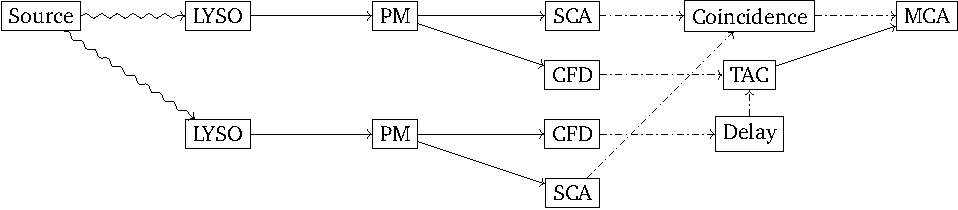
\includegraphics{fast-slow}
    \caption{%
        Schematic of the fast-slow circuit. Wavy lines are photons, solid lines
        analog signal and dash-dotted lines denote digital pulses.
    }
    \label{fig:fast-slow}
\end{figure}

The start photon will be detected in the upper LYSO detector and amplified by
the photomultiplier (PM). The signal from the last dynode is amplified and fed
into the upper SCA\@. If the amplitude (i.e.\ the photon energy) matches, the SCA
emits a long rectangular pulse to the coincidence unit. The fast signal from
the same photomultiplier is given to a CFD\@. This upper CFD will trigger the
start on the TAC\@.

A short time later, when the positron has decayed, a
\SI{511}{\kilo\electronvolt} photon will reach the other LYSO detector. The
same outputs are used and fed to the lower SCA and CFD, respectively.
Overlapping with the pulse of the upper SCA, the lower SCA will emit a
rectangular pulse as well. Both pulses match in the coincidence unit and open
the gate on the MCA\@. The output of the lower CFD is delayed to make sure that
it arrives later at the TAC\@.

Once the stop signal arrived at the TAC, the latter will emit an analog pulse
to the MCA which is proportional to the duration between start and stop. In the
MCA a histogram of durations is therefore built up.

\subsection{Prompt curve}

The bins in the MCA histogram do not have any time scale associated with them,
a time gauge needs to be derived first. For this we use that electrons and
positrons decay into two back-to-back photons when their net spin is zero. We
can set both SCA windows to the typical \SI{511}{\kilo\electronvolt} energy and
assume that both photons are emitted simultaneously. We expect to measure a
duration of \SI{0}{\nano\second} plus the explicit delay. On the MCA this
should give a sharp peak which marks our zero. Adding more time to the delay
will shift this peak in the histogram. The distance of the peaks will give us
the relation between duration and histogram bins. This process will be done
several times for statistical accuracy.

\section{Analysis models}

\subsection{Lifetime spectrum}

As in Section~\ref{ssec:tra_mod} stated the lifetime spectrum contains a
superposition of two decays with different lifetimes $\tau_0$ and
$\tau_\text{t}$ and their corresponding relative intensities $I_0$ and
$I_\text{t}$:
\begin{align*}
        W (t) &= \frac{I_0}{\tau_0}\eup^{-\frac{t}{\tau_0}} +
        \frac{I_t}{\tau_t}\eup^{-\frac{t}{\tau_t}}.
        \intertext{%
                For the detecting system has a limited time resolution the
                obtained spectrum is a convolution of the real lifetime
                spectrum with the resolution function:
        }
        M (t) &= (W * P)(t) \\
              &= \sum_{i\in\{0,\text{t}\}}\frac{I_0}{2\tau_i}
        \exp\!\del{\frac{\sigma^2-2\tau_i(t-t_0)}{2\tau_i^2}}
        \del{\text{erf}\!\del{\frac{\sigma^2 + \tau_it_0} {\sqrt2\sigma\tau_i}}
        + \text{erf}\!\del{\frac{\tau_i(t-t_0)-\sigma^2}{\sqrt2\sigma\tau_i}}},
        \intertext{%
                with $\text{erf}(x)$ being the Gaussian error function. For
                fitting data, where we have a background $N_\text{BG}$, we use
        }
        N (t) &= \sum_{i\in\{0,\text{t}\}}\frac{A_i}{2\tau_i}
        \exp\!\del{\frac{\sigma^2-2\tau_i(t-t_0)}{2\tau_i^2}}
        \del{\text{erf}\!\del{\frac{\sigma^2 + \tau_it_0} {\sqrt2\sigma\tau_i}}
        + \text{erf}\!\del{\frac{\tau_i(t-t_0)-\sigma^2}{\sqrt2\sigma\tau_i}}}
        \\
        & + N_\text{BG}.
        \intertext{%
                The count amplitudes $A_0$ and $A_\text{t}$ are related to the
                intensities by
        }
        I_i &= \frac{A_i}{A_0 + A_\text{t}}.
\end{align*}

\subsection{Arrhenius plot}

\chapter{Procedure and Analysis}

\section{Slow circuit setup}

\subsection{LYSO spectrum}

Before adjusting the amplifiers, we have to associate the detected events with
the corresponding transitions. To separate the decay of the ${}^{22}\text{Na}$
from the intrinsic \textsc{lyso} spectrum, we first take the \textsc{lyso}
spectrum of the left and right detectors. In Figure~\ref{fig:lyso} one can
clearly determine the $\SI{596.82}{\kilo\electronvolt}$ cascade decay of the
$6^+$ state of ${}^{176}\text{Hf}$.

\begin{figure}
        \centering
        \begin{subfigure}[c]{.49\linewidth}
                \centering
                \includegraphics{lyso-li}
                \caption{%
                        Left detector.
                }
                \label{fig:lyso-li}
        \end{subfigure}
        \hfill
        \begin{subfigure}[c]{.49\linewidth}
                \centering
                \includegraphics{lyso-re}
                \caption{%
                        Right detector.
                }
                \label{fig:lyso-re}
        \end{subfigure}
        \caption{%
                Intrinsic energy spectrum of the \textsc{lyso} detector.
        }
        \label{fig:lyso}
\end{figure}
        

\subsection{Gain adjust using sodium}

In the sodium spectrum, we expect to see the \SI{511}{\kilo\electronvolt} line
from the annihilation as well as a \SI{1275}{\kilo\electronvolt} line from the
excited neon.

We adjust the gain of the amplifiers such that the sodium spectrum fill the
8192 channels of the \textsc{mca}. The maximum window width of the \textsc{sca}
is not sufficient to let everything through. Also the upper bound for the
\textsc{sca} is below the last channel of the \textsc{mca}. Therefore we cannot
set the amplifier as high as we would like to. For the spectrum, we adjust the
lower bound such that the window covers the two lines we are interested. The
spectra of the left and the right detector are shown in
Figure~\ref{fig:natrium}.

\begin{figure}
        \centering
        \begin{subfigure}[c]{.49\linewidth}
                \centering
                \includegraphics{na-li}
                \caption{%
                        Left detector.
                }
                \label{fig:na-li}
        \end{subfigure}
        \hfill
        \begin{subfigure}[c]{.49\linewidth}
                \centering
                \includegraphics{na-re}
                \caption{%
                        Right detector.
                }
                \label{fig:na-re}
        \end{subfigure}
        \caption{%
                Spectrum of ${}^{22}\text{Na}$. The lines of the detector
                material are also visible.
        }
        \label{fig:natrium}
\end{figure}


We check the coincidence of both \textsc{sca} signals.

\section{Fast circuit setup}

Slow-signal and CFD signal, adjust CFD such that zero-line vanishes.

Look at CFD signals where stop-signal is delayed. We can verify that there is a
\SI{20}{\milli\second} delay between the two.

TAC produces an output.

\section{Time calibration}

SCA coincidence already checked.

TAC+coincidence has very nice overlap.

For a time calibration of our \textsc{mca} we use the coincidence unit as
\textsc{mca}-gate and the \textsc{tac} as input, to take six prompt curves.
Between the measurements another \SI{4}{\nano\second}-delay is interposed. For
the first five prompt curves an acquisition time of about \SI{2}{\minute} is
used.  Together with their fitted Gauss-curves they are shown in
Figure~\ref{fig:prompts_short}. The sixth prompt curve and its fit is shown in
Figure~\ref{fig:prompts_long}. To get a good estimation of the time resolution
the acquisition time is \SI{20}{\minute}.

\begin{figure}
\centering
        \includegraphics{prompts_short}
        \caption{%
                Prompt curves for time calibration. Acquisition time for every
                curve is approximately \SI{2}{\minute}.
        }
        \label{fig:prompts_short}
\end{figure}
        
\begin{figure}
\centering
        \includegraphics{prompts_long}
        \caption{%
                Additional prompt curve for time calibration and time
                resolution estimation. Acquisition time is approximately
                \SI{20}{\minute}.
        }
        \label{fig:prompts_long}
\end{figure}

From the fitted functions we get the mean channel to every delay time. The
results are in Table~\ref{tab:time_gauge_param}. If one plots delay time
against channel number (see Fig.~\ref{fig:time_gauge}) one gets a linear
correlation. Because we don't need absolute time values, just time differences,
only the slope of the fit is of interest for us, which is \SI{<<
time_gauge_slope >>}{\milli\second}.

\begin{table}
        \centering
        \begin{tabular}{SS}
                \toprule
                {delay time/\si{\nano\second}}
                & {mean channel number} \\
                \midrule
                %< for row in time_gauge_param >%
                << ' & '.join(row) >> \\
                %< endfor >%
                \bottomrule
        \end{tabular}
        \caption{%
                Mean channel number of Gauss fit width corresponding delay
                times.
        }
        \label{tab:time_gauge_param}
\end{table}

\begin{figure}
        \centering
        \includegraphics{time_gauge}
        \caption{%
                Time calibration of \textsc{mca}-channels. The error bars for
                the channel number are so small, they hide behind the
                markers.
        }
        \label{fig:time_gauge}
\end{figure}
        

The last prompt curve has a standard deviation of \num{<< width_6 >>}. From
this we get $\textsc{fwhm} = \num{<< FWHM_6 >>}$. With the slope of the time
calibration fit we get a resolution of \SI{<< time_resolution >>}{\nano\second}.

\section{Adjusting SCA windows}

After the time calibration we have to set up the fast-slow coincidence
circuit. For this we set the \textsc{sca} window on the start-side
to the \SI{1275}{\kilo\electronvolt} line of the spectrum and check if the
two \textsc{sca}'s as well as the \textsc{tac} and the coincidence unit have
a nice overlap.

\section{Indium sample}

An indium sample is placed inside an aluminum block, which is mounted on a
soldering iron. This allows us to control the sample's temperature with an
potentiometer. A thermometer enables us to read off the actual temperature. Now
the sample is placed between the detectors, which have to be shielded against
the heat by two aluminum plates. We have to ensure that there is no contact to
the heat shielding. 

\subsection{Lifetime spectrum}

The first measurement is at room temperature. After about \SI{30}{\minute} we
stop the event recording at the computer and save the data. Then we turn up the
temperature and wait for the temperature to reach a nearly
constant value. We repeat this untill we have eight data sets. For every
measurement we note the temperature in the beginning and at the end of the
acquisition.

The measurement at room temperature together with a fit function is shown in
Figure~\ref{fig:lifetime-295K}. For the other measurements see
Figures~\ref{fig:lifetime-324K}~to~\ref{fig:lifetime-398K} in the appendix.

\begin{figure}
    \centering
    \includegraphics{lifetime-295K}
    \caption{%
        Lifetime spectrum of indium at room temperature.
    }
    \label{fig:lifetime-295K}
\end{figure}

\begin{figure}
    \centering
    \includegraphics{taus}
    \caption{%
        Compilation of the various lifetimes derived from the spectra.
    }
    \label{fig:taus}
\end{figure}

\begin{figure}
    \centering
    \includegraphics{s_curve}
    \caption{%
        $\bar\tau$ against the temperature. One would expect to see an
        \enquote{S}-shape here.
    }
    \label{fig:s_curve}
\end{figure}

\subsection{Vacancy formation enthalpy}

\begin{figure}
    \centering
    \includegraphics{arrhenius}
    \caption{%
        %
    }
    \label{fig:arrhenius}
\end{figure}

\section{Acrylic glass sample}

\begin{appendix}

    \chapter{Lifetime spectra}

    %TODO insert temperatures
    \begin{figure}
        \centering
        \includegraphics{lifetime-324K}
        \caption{%
            Lifetime spectrum of indium at room temperature.
        }
        \label{fig:lifetime-324K}
    \end{figure}

    \begin{figure}
        \centering
        \includegraphics{lifetime-339K}
        \caption{%
            Lifetime spectrum of indium at room temperature.
        }
        \label{fig:lifetime-339K}
    \end{figure}

    \begin{figure}
        \centering
        \includegraphics{lifetime-350K}
        \caption{%
            Lifetime spectrum of indium at room temperature.
        }
        \label{fig:lifetime-350K}
    \end{figure}

    \begin{figure}
        \centering
        \includegraphics{lifetime-362K}
        \caption{%
            Lifetime spectrum of indium at room temperature.
        }
        \label{fig:lifetime-362K}
    \end{figure}

    \begin{figure}
        \centering
        \includegraphics{lifetime-376K}
        \caption{%
            Lifetime spectrum of indium at room temperature.
        }
        \label{fig:lifetime-376K}
    \end{figure}

    \begin{figure}
        \centering
        \includegraphics{lifetime-388K}
        \caption{%
            Lifetime spectrum of indium at room temperature.
        }
        \label{fig:lifetime-388K}
    \end{figure}

    \begin{figure}
        \centering
        \includegraphics{lifetime-398K}
        \caption{%
            Lifetime spectrum of indium at room temperature.
        }
        \label{fig:lifetime-398K}
    \end{figure}

\end{appendix}

\end{document}

% vim: spell spelllang=en_us tw=79
